\subsubsection{Test case II: \texorpdfstring{$\phi^4$}{phi**4} theory}
\label{subsubsec:sc2}
The \textit{test case II} is a zero-dimensional version of $\phi^4$ theory with the \uv{} initial potential
	\begin{align}
		U ( \vec{\varphi} \vts ) = \mp \tfrac{1}{2} \, \vec{\varphi}^{\vts 2} + \tfrac{1}{4!} \, ( \vec{\varphi}^{\vts 2} )^2 \, ,	\label{eq:testing_scenario_phi4}
	\end{align}
where a theory with negative mass term $-\tfrac{1}{2} \, \vec{\varphi}^{\vts 2}$ has a \textit{``sombrero''}-type (symmetric double-well) potential well-known from standard textbook discussions of spontaneous symmetry breaking~\cite{Goldstone:1961eq,Goldstone:1962es}.
The corresponding \ic{} with negative mass term for the \frg{} flow is illustrated in \cref{fig:sc_ii_n_uv_initial_condition}.
When not explicitly stated otherwise we will consider the \ic{} \eqref{eq:testing_scenario_phi4} with negative mass term.
The reference values for the exact \ir{} \ipi{} vertex functions $\Gamma^{(2n)}$ of the $O(N)$ model \eqref{eq:on-model_relation_2pf_phi2}\nolinebreak[3]--\nolinebreak[2]\eqref{eq:on-model_relation_6pf_phi2} are calculated numerically from the \uv{} potential \eqref{eq:testing_scenario_phi4} and are listed for selected values of $N$ in \cref{tab:sc_2_n_point_functions_exact} both for positive and negative mass terms.

In the remainder of this subsubsection we will use test case II to discuss
\begin{itemize}
	\item \customref{paragraph:sc2KT}{Results obtained using the KT scheme},
	\item \customref{paragraph:sc2taylorFlow}{FRG Taylor expansion: Flow of the \nptFunctions{}},
	\item \customref{paragraph:sc2taylorError}{FRG Taylor expansion: Truncation error},
	\item \customref{paragraph:sc2taylorPhiP}{FRG Taylor expansion: $\phi^4$ potential with positive mass term},
	\item \customref{paragraph:sc2taylorIRR}{FRG Taylor expansion: Numerical irreversibility},
\end{itemize}
in the corresponding paragraphs which are based on Secs.~V.B.1\dash{}2 of \nbccite{zerod1}.
\fullWidthTwoColumnFigureTable%
	[!t] % Placement
	{0d/figures/sc_ii_n_uv_initial_condition.pdf} % Figure
	{fig:sc_ii_n_uv_initial_condition} % Figure label
	{%
		\uv{} potential $U ( \sigma )$ (red-dashed) and its first derivative $u ( \sigma ) = \partial_\sigma U ( \sigma )$ (blue, solid) of test case II from \cref{eq:testing_scenario_phi6} with negative mass term. 
		\fromFig{18}{zerod1}%
	} % Figure caption
	{%
		\renewcommand{\arraystretch}{1.15}
		\small
		\begin{tabular}{l c c c}
			\toprule
			$N$		&	$\Gamma^{(2)}$	&	$\Gamma^{(4)}$	&	$\Gamma^{(6)}$	\\
			\midrule
				$1$	&	$0.199510$	&	$0.062258$	&	$0.107744$\\
				$4$	&	$0.506444$	&	$0.182415$	&	$0.280288$\\
				\hline
				$1^{*}$	&	$1.332430$	&	$0.607899$	&	$0.771451$\\
				$4^{*}$	&	$1.580920$	&	$0.611848$	&	$0.568631$\\
			\bottomrule
		\end{tabular}
	} % Table content
	{tab:sc_2_n_point_functions_exact}% Table label
	{%
		Exact results for $\Gamma^{(2n)}$ of the $O(N)$ model with the \uv{} initial potential \eqref{eq:testing_scenario_phi4} for selected $N$  with negative and positive${}^{*}$ mass term.
		They are obtained by a high-precision one-dimensional numerical integration of the expectation values $\langle ( \vec{\phi}^{\, 2} )^n \rangle$ from \cref{eq:ON_expectation_value} using \textit{NIntegrate} in \WAMXIIwR{}.
		Here, we present the first six digits only.
		\textit{In parts from Tab. II of \ccite{zerod1} and Tab. I of \nbccite{zerod2}.}%
	} % Table caption
\FloatBarrier
\paragraph{Results obtained using the \ktScheme{}}\phantomsection\label{paragraph:sc2KT}\mbox{}\\%
\fullWidthTwoColumnFigures%
	[!t] % Placement
	{%
		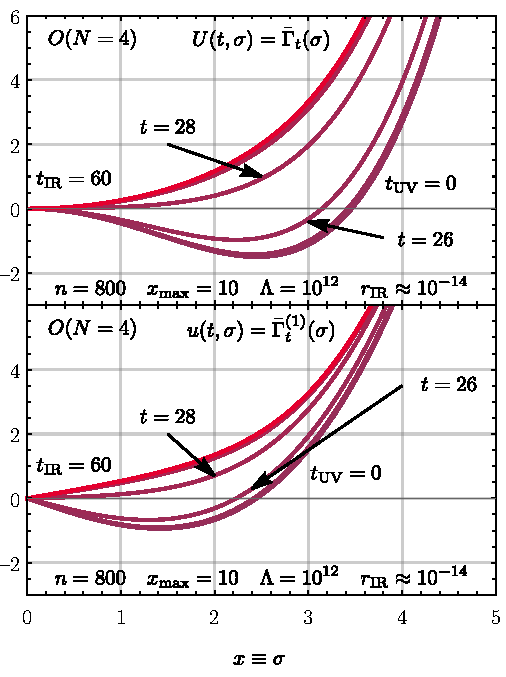
\includegraphics[width=\subcaptionFigureWidth-0.17cm]{0d/figures/sc_ii_n_on_4_n_800_xmax_10_lambda_1e12_tir_60_rg_flow.pdf} % left figure
		\captionsetup{width=\subcaptionFigureWidth-0.17cm}%
		\caption{
			The \frg{} flow of the effective potential $U ( t, \sigma )$ (upper panel) and its derivative $u ( t , \sigma ) = \partial_\sigma U ( t , \sigma )$ (lower panel) for the zero-dimensional $O ( 4 )$ model with \ic{} \eqref{eq:testing_scenario_phi4}, evaluated at $t = 0, \, 2, \, 4, \, \ldots, \, 60$ (integer values for $t$ were chosen for convenience and readability). 
			The (overlapping) {blue} and {violet} curves correspond to the \uv{} and the {red} curves to the \ir{}.
			We used the exponential regulator~\eqref{eq:exponential_regulator} with \uv{} scale $\Lambda = 10^{12}$.
			The plot does not show the region ${x \in[5,10]}$, because the tiny differences between $u ( t, \sigma )$ and $u ( t_\mathrm{UV}, \sigma )$ are not visible in this region and vanish for large $x = \sigma$ anyhow.
			\fromFig{19}{zerod1}
		}
		\label{fig:sc_ii_n_on_4_n_800_xmax_10_lambda_1e12_tir_60_rg_flow}%
	}
	{\fullWidthTwoColumnFigureSpacing}
	{
		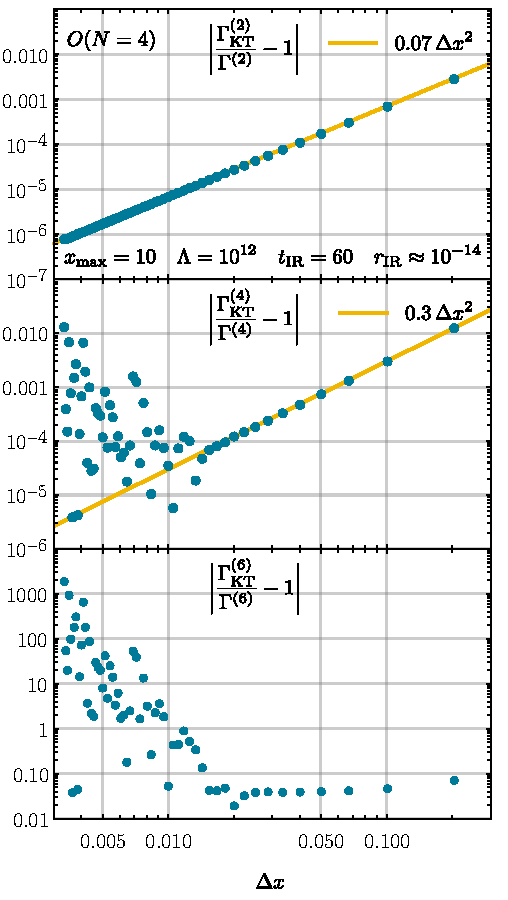
\includegraphics[width=\subcaptionFigureWidth+0.17cm]{0d/figures/sc_ii_n_on_4_xmax_10_lambda_1e12_tir_60_deltax_scaling.pdf} % Right figure
		\captionsetup{width=\subcaptionFigureWidth-0.17cm}%
		\caption{%
			The relative error as a function of the cell size $\Delta x$ for the numerical results (blue dots) from the KT scheme for the coefficients $\Gamma^{(2n)}$ for $n = 1, 2, 3$ with initial potential \eqref{eq:testing_scenario_phi4}.
			The numerical derivatives at $\sigma = 0$ of $u ( t_\mathrm{IR} = 60, \sigma )$ were calculated via the second-order accurate central schemes \eqref{eq:derivative_1_central_error_2}, \eqref{eq:derivative_3_central_error_2}, and \eqref{eq:derivative_5_central_error_2}.
			Here, $x_\mathrm{max} = 10$, but we could have used any sufficiently large $x_\mathrm{max}$.
			We used the exponential regulator~\eqref{eq:exponential_regulator} with \uv{} scale $\Lambda = 10^{12}$.
			The yellow straight lines $\propto \Delta x^2$ are for optical guidance.
			\fromFig{21}{zerod1}%
		}%
		\label{fig:sc_ii_n_on_4_xmax_10_lambda_1e12_tir_60_deltax_scaling}%
	}
In this paragraph we will discuss selected numerical results of the application of the \ktScheme{} for the analytic \ic{} \eqref{eq:testing_scenario_phi4}.
We have performed the full set of numerical tests discussed in \cref{subsubsec:sc1} for this \ic{} and found results supporting the general statements made there.
For brevity, we will not repeat the complete discussion of that subsubsection.
We will limit our discussion to \uv{}/\ir{} scales, the computational domains size ($x_\mathrm{max}$), and its resolution ($\Delta x$). \bigskip

\textbf{\uv{} and \ir{} scales:}
In \cref{fig:sc_ii_n_on_4_n_800_xmax_10_lambda_1e12_tir_60_rg_flow} we present the \frg{} flow of the derivative of the effective potential $u ( t, \sigma )$ from the \uv{} ({blue}) to the \ir{} ({red}).
For the smooth \ic{} \dash{} in the absence of large gradients \dash{} the highly non-linear advection and diffusion contribute almost an equal amount to the dynamics.
Between $t \approx 25$ and $t \approx 30$ we observe significant changes in the shape of the potential: the non-trivial minimum moves towards $\sigma = 0$ and vanishes at $t \approx 28$ resulting in a convex potential with a trivial minimum at $\sigma = 0$ as expected and required.
At small and large $t$ outside the apparent dynamic range between $t \approx 25$ and $t \approx 30$ we observe only very marginal changes in \cref{fig:sc_ii_n_on_4_n_800_xmax_10_lambda_1e12_tir_60_rg_flow}.

A close inspection of the relative errors for the first three non-vanishing \nptFunctions{} in \cref{fig:sc_ii_n_on_4_n_400_xmax_10_lambda_1e12_tir_60_flow_errors} reveals that actually the relevant dynamics sets in much earlier at $t \approx 10$ for the six-point function.
The values for the \nptFunctions{} freeze out at late times around $t \approx 40$, which is due to the diffusion close to $\sigma = 0$.
On the level of $u ( t, \sigma )$ these subtle changes in the \nptFunctions{} cannot be observed by a simple visual inspection of \cref{fig:sc_ii_n_on_4_n_800_xmax_10_lambda_1e12_tir_60_rg_flow}.

The plateaus in the \uv{} (at small $t$) and the \ir{} (at large $t$) support the choice of $\Lambda=10^{12}$ and $t_\mathrm{IR}=60$ to be valid initial \uv{} and \ir{} cutoff scales in terms of \rgcy{}. 
The present \uv{} initial scale is larger when compared to $\Lambda=10^{6}$, which corresponds to $t \approx 14$ in the dynamic region in \cref{fig:sc_ii_n_on_4_n_400_xmax_10_lambda_1e12_tir_60_flow_errors}, used for most computations involving the non-analytic potential considered in the previous \cref{subsubsec:sc1}. 

Hence, the inclusion of a quartic interaction term in \cref{eq:testing_scenario_phi4} seems to require higher \uv{} initial scales to ensure \rgcy{}.
This supports the  statements made in \cref{paragraph:ONRGconsistency}: \rgcy{} and \uv{}/\ir{} scales have to be re-evaluated when changing the \ic{} in the \uv{}, \ie{}, the model under consideration, since characteristic internal scales then also change.\bigskip

\fullWidthTwoColumnFigures%
	[!t] % Placement
	{%
		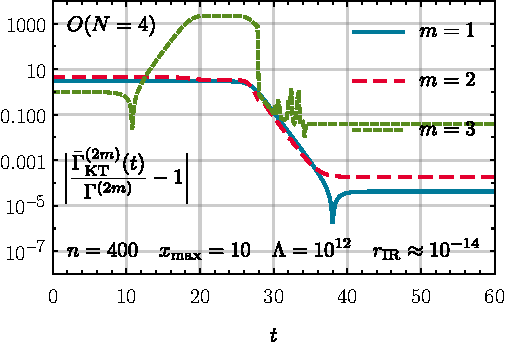
\includegraphics[width=\subcaptionFigureWidth-0.04cm]{0d/figures/sc_ii_n_on_4_n_400_xmax_10_lambda_1e12_tir_60_flow_errors.pdf} % left figure
		\captionsetup{width=\subcaptionFigureWidth-0.04cm}%
		\caption{%
			The relative error for $\Gamma^{(2m)}$, for $m = 1, 2, 3$, calculated with the \ktScheme{} as a function of the \rgtime{} $t$ for the $O(4)$ model.
			The \uv{} initial potential is given by \cref{eq:testing_scenario_phi4}.
			We use the exponential regulator~\eqref{eq:exponential_regulator} with \uv{} scale $\Lambda = 10^{12}$.
			The computational grid has $n=400$ cells and $\sigma_\mathrm{max} = x_\mathrm{max} = 10$.
			$\Gamma^{(2m)}$ are extracted from $u ( t_\mathrm{IR} = 60, \sigma )$ via the finite-difference stencils \eqref{eq:derivative_1_central_error_2}, \eqref{eq:derivative_3_central_error_2}, and \eqref{eq:derivative_5_central_error_2}.
			\fromFig{20}{zerod1}
		}
		\label{fig:sc_ii_n_on_4_n_400_xmax_10_lambda_1e12_tir_60_flow_errors}
	}
	{\fullWidthTwoColumnFigureSpacing}
	{%
		\vspace{-0.2cm}
		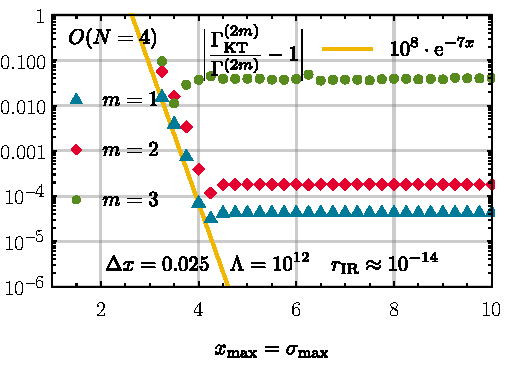
\includegraphics[width=\subcaptionFigureWidth+0.04cm]{0d/figures/sc_ii_n_on_4_deltax_25e-3_lambda_1e12_tir_60_errors_xmax.pdf} % Right figure
		\captionsetup{width=\subcaptionFigureWidth+0.04cm}%
		\caption{%
			The relative error for $\Gamma^{(2m)}$ for $m = 1, 2, 3$ for the \uv{} potential \eqref{eq:testing_scenario_phi4} of the $O ( 4 )$ model as a function of $x_\mathrm{max}$, keeping the cell size $\Delta x = 0.025$ constant.
			$\Gamma^{(2m)}$ are computed from the discrete values of the derivative of the \ir{} potential $u ( t_\mathrm{IR} = 60, \sigma )$ via the second-order accurate central finite-difference stencils \eqref{eq:derivative_1_central_error_2}, \eqref{eq:derivative_3_central_error_2}, and \eqref{eq:derivative_5_central_error_2} at $\sigma = 0$.
			We used the exponential regulator~\eqref{eq:exponential_regulator} with \uv{} scale $\Lambda = 10^{12}$.
			The yellow straight line $\propto\exp\del{-7\,x_\mathrm{max}}$ is for optical guidance.
			\fromFig{22}{zerod1}%
		}%
		\label{fig:sc_ii_n_on_4_deltax_25e-3_lambda_1e12_tir_60_errors_xmax}
	}
\textbf{Size and resolution of the computational domain:} We conclude this paragraph on the \kt{} scheme with a brief discussion regarding the computational domain.
The relative error for the first three non-vanishing \nptFunctions{} is shown as a function of the cell size $\Delta x$ in \cref{fig:sc_ii_n_on_4_xmax_10_lambda_1e12_tir_60_deltax_scaling}.
For the two-point function we recover a perfect error scaling with $\Delta x^2$ down to extremely small $\Delta x$.
The last data point in \cref{fig:sc_ii_n_on_4_xmax_10_lambda_1e12_tir_60_deltax_scaling} is at ${\Delta x \approx 3.3 \cdot 10^{-3}}$ corresponding to $n=3000$ cells.
For the two-point function the rounding errors of the employed finite-difference extraction \eqref{eq:derivative_1_central_error_2} for $\Gamma^{(2)}$ and the finite precision of the \ode{} integrator (\textit{NDSolve} from \WAMXIIwR{} with a \textit{PrecisionGoal} and \textit{AccuracyGoal} of $10$) seem to be small for all depicted $\Delta x$ in this scenario. 
A comparison with the present perfect error scaling for $\Gamma^{(2)}$ supports the comments made about discretization errors for the discontinuous \ic{} \eqref{eq:testing_scenario_non-analytic_quadaratic_asymptote} in \cref{fig:sc_i_on_3_xmax_10_lambda_1e6_tir_60_deltax_scaling}.
For the higher-order \nptFunctions{} $\Gamma^{(4)}$ and $\Gamma^{(6)}$, however, we find that rounding errors related to the finite-difference extractions \eqref{eq:derivative_3_central_error_2} and \eqref{eq:derivative_5_central_error_2} limit the achievable precision.
Again, we identify $\Delta x \approx 0.025$ as an optimal cell size for the extraction of $\Gamma^{(4)}$ and $\Gamma^{(6)}$ but note that typical relative errors for $\Gamma^{(6)}$ are at $\approx 4 \%$ around $\Delta x \approx 0.025$.

In \cref{fig:sc_ii_n_on_4_deltax_25e-3_lambda_1e12_tir_60_errors_xmax}, we study the effect of the size of the computational domain $x_\mathrm{max}$ on the achievable relative errors for $\Gamma^{(2)}$, $\Gamma^{(4)}$, and $\Gamma^{(6)}$ at a constant $\Delta x =0.025$. 
One major difference between the $\phi^4$ potential \eqref{eq:testing_scenario_phi4} studied in this subsubsection and the non-analytic potential~\eqref{eq:testing_scenario_non-analytic_quadaratic_asymptote} of the previous \cref{subsubsec:sc1} is their asymptotic behavior for large $\sigma$.
For large $\sigma$ the leading-order term of the $\phi^4$ potential is \dash{} as the name suggests \dash{} quartic while the non-analytic potential of test case I grows only quadratic.
In terms of the conserved quantity $u = \partial_\sigma U$ one might expect problems when using a linear extrapolation for the ghost cells at large $\sigma$ as discussed in \cref{paragraph:BCinf} with a potential where $u$ grows $\sim \sigma^3$ for large $\sigma$.
For the non-analytic \ic{} \eqref{eq:testing_scenario_phi4} we avoided this possible source of error by construction.
However, considering the results plotted in \cref{fig:sc_ii_n_on_4_deltax_25e-3_lambda_1e12_tir_60_errors_xmax} together with the perfect error scaling displayed in the previous \cref{fig:sc_ii_n_on_4_xmax_10_lambda_1e12_tir_60_deltax_scaling}, we conclude that a linear extrapolation is not problematic even in the case of cubic asymptotics for $u$.
This might be again in part related to the large spatial distance between the physical minimum in the \ir{} and the upper boundary of the grid.
For $x_\mathrm{max}\smallergtrsim 5$ we find a complete insensitivity of the relative errors on the interval size.

\FloatBarrier
\paragraph{\frg{} Taylor expansion: Flow of the $n$-point vertex functions}\phantomsection\label{paragraph:sc2taylorFlow}\mbox{}\\
In this paragraph we confront the theoretical results and concerns stated in \teRef{} and especially in \cref{subsubsec:vertex_expansion} for the zero-dimensional $O(N)$ model \wrt{} the Taylor expansion around the fixed expansion point $\vec{\varphi} = 0$ with the exact results for the zero-dimensional $O(N)$ model.
The $\phi^4$ potential of \cref{eq:testing_scenario_phi4} with negative mass term is the, in terms of \ics{}, simplest \uv{} potential with a non-trivial minimum.
At the end of this subsection we will briefly discuss the Taylor expansion for the $\phi^4$ potential with positive mass term and therefore a scenario without a non-trivial minimum, which has to be considered the simplest non-trivial, \ie{}, interacting, \uv{} \ic{} in the context of the Taylor expansion for the zero-dimensional $O(N)$ model.

In the following we integrate the \ode{} system \eqref{eq:example_vertex_expansion} truncated at $m = 2 n_\mathrm{trunc}$ with the \ic{}
\begin{align}
	\bar{\Gamma}^{(2)} ( 0 ) = - 1 \, ,\qquad \bar{\Gamma}^{(4)} ( 0 ) = + 1 \, ,\qquad \forall n > 2 \quad \bar{\Gamma}^{(2n)} ( 0 ) = 0 \, ,
\end{align}
corresponding to the potential \eqref{eq:testing_scenario_phi4} numerically up to $t_\mathrm{IR}=60$ employing the exponential regulator~\eqref{eq:exponential_regulator} with $\Lambda=10^{12}$ and using the same \ode{} solver \textit{NDSolve} from \WAMXIIwR{} with a \textit{PrecisionGoal} and \textit{AccuracyGoal} of $10$ as before.
Using the \nptFunctions{} at the physical minimum as the flow variables makes an additional extraction procedure (like \acrpllong{fd}) obviously obsolete.
The \nptFunctions{} in the \ir{} can be directly obtained from the values $\bar{\Gamma}^{(2n)} ( t_\mathrm{IR} ) = \Gamma^{(2n)}$.

\fullWidthTwoColumnFigures%
	[!t] % Placement
	{%
		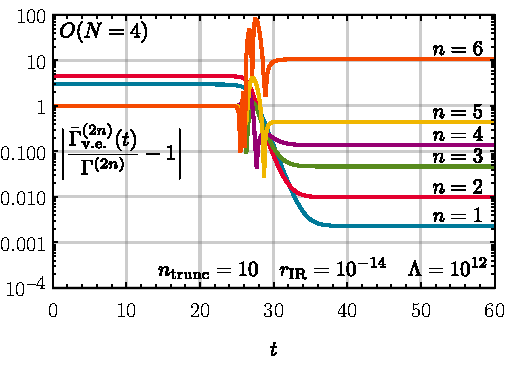
\includegraphics[width=\subcaptionFigureWidth]{0d/figures/sc_ii_n_on_4_lambda_1e12_tir_60_ntrunc_10_vertex_exp_flow.pdf} % left figure
		\captionsetup{width=\subcaptionFigureWidth}%
		\caption{%
			The relative errors for $\Gamma^{(2n)}$ as a function of the \rgtime{} $t$ for $n \in \{ 1, \ldots, 6 \}$ for the $O (4)$ model.
			$\Gamma^{(2n)}$ were calculated via the \frg{} flow of the \frg{} Taylor expansion with truncation order $m = 2 n_\mathrm{trunc} = 20$ using the exponential regulator~\eqref{eq:exponential_regulator}. 
			As initial condition we use the \uv{} potential \eqref{eq:testing_scenario_phi4}.
			\fromFig{23}{zerod1}
		}
		\label{fig:sc_ii_n_on_4_lambda_1e12_tir_60_ntrunc_10_vertex_exp_flow}
	}
	{\fullWidthTwoColumnFigureSpacing}
	{%
		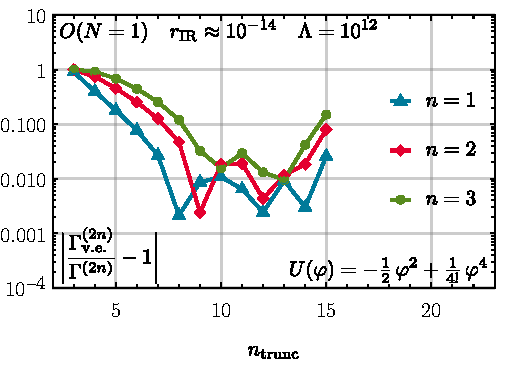
\includegraphics[width=\subcaptionFigureWidth]{0d/figures/sc_ii_n_on_1_lambda_1e12_tir_60_vertex_exp_error.pdf} % Right figure
		\captionsetup{width=\subcaptionFigureWidth}%
		\caption{%
			The relative errors for $\Gamma^{(2n)}$ in the \ir{} for $n = 1, 2, 3$ for the $O (1)$ model, calculated via the \frg{} flow of the \frg{} Taylor expansion to order $m = 2 n_\mathrm{trunc}$ with $n_\mathrm{trunc} \in \{ 3, \ldots , 15 \}$ using the exponential regulator~\eqref{eq:exponential_regulator}.
			As initial condition we use the \uv{} potential \eqref{eq:testing_scenario_phi4}.
			The discrete results for integer $n_\mathrm{trunc}$ are connected by straight lines to improve readability and for a better trend analysis.
			\fromFig{25}{zerod1}%
		}%
		\label{fig:sc_ii_n_on_1_lambda_1e12_tir_60_vertex_exp_error}
	}%
In \cref{fig:sc_ii_n_on_4_lambda_1e12_tir_60_ntrunc_10_vertex_exp_flow} we show the flow of the relative deviations for the first six non-vanishing \nptFunctions{} towards the \ir{} using $m = 2 n_\mathrm{trunc} = 20$ vertices in the expansion for the $O(4)$ model.
We can identify a dynamic range between $t \approx 24$ and $t \approx 38$ in which the vertices vary significantly and change their signs before they reach their respective \ir{} values.
This range is substantially smaller than the dynamic range observed when solving the full \pde{} \eqref{eq:conservation_law_u_phi} using the \ktScheme{}, \cf{} \cref{fig:sc_ii_n_on_4_n_400_xmax_10_lambda_1e12_tir_60_flow_errors}.
In the \ir{}, the errors range from $2.3 \cdot 10^{-3}$ for $\Gamma^{(2)}$ to $1.1 \cdot 10^{1}$ for $\Gamma^{(12)}$.
However, the strict hierarchy observed in \cref{fig:sc_ii_n_on_4_lambda_1e12_tir_60_ntrunc_10_vertex_exp_flow} for $n = 1, \ldots, 6$ is not a general feature of the Taylor expansion for this model.
Using different $n_\mathrm{trunc}$ or including higher-order vertices changes this hierarchy.

\paragraph{\frg{} Taylor expansion: Truncation error}\phantomsection\label{paragraph:sc2taylorError}\mbox{}\\
The truncation error for the $O(4)$ model is discussed using \cref{fig:sc_ii_n_on_4_lambda_1e12_tir_60_vertex_exp_error}, where we show the relative errors for $\Gamma^{(2)}$, $\Gamma^{(4)}$, and $\Gamma^{(6)}$ for the Taylor expansion using different truncation orders $m=2n_\mathrm{trunc}$ between $n_\mathrm{trunc}=3$ and $n_\mathrm{trunc}=14$. 
Beyond $n_\mathrm{trunc}=10$ the relative errors for the \nptFunctions{} no longer decrease and we observe rather strong oscillations for different $n_\mathrm{trunc}$.
The errors for the two and four-point function are with $2.3 \cdot 10^{-3}$ and $9.8 \cdot 10^{-3}$ larger than the errors ($4.2 \cdot 10^{-5}$ and $1.8 \cdot 10^{-4}$ respectively) obtained in the \ktScheme{}, see,  \eg{}, \cref{fig:sc_ii_n_on_4_deltax_25e-3_lambda_1e12_tir_60_errors_xmax}. 
The relative error for the six-point function is with $4.7 \cdot 10^{-2}$ comparable to the $3.7 \cdot 10^{-2}$ error obtained in the \ktScheme{}.
While the extraction of higher-order \nptFunctions{} beyond $n = 6$ is in general possible in the Taylor expansion, their relative errors grow overall rapidly with increasing $n$.

For the \ic{} \eqref{eq:testing_scenario_phi4} we do not observe any meaningful error scaling in orders of $n_\mathrm{trunc}$.
Furthermore a numerical solution at and beyond $n_\mathrm{trunc}=15$ has proven impossible with the current set-up.
At $n_\mathrm{trunc}=15$ an \ode{} integration to the \ir{} at $r ( t_\mathrm{IR} = 60 ) \approx 10^{-14}$ is impossible due to an instability of the \ode{} system occurring at $t \approx 30$ where all coefficients $\Gamma^{(2n)}(t)$ with $n>1$ start diverging.
This divergence seems to be driven by $\Gamma^{(30)}(t)$ for $n_\mathrm{trunc}=15$.
The \ode{} system is in general poorly conditioned since the $\Gamma^{(2n)}(t)$ for different $n$ vary vastly over multiple orders of magnitude.
The instability at  $t \approx 30$ cannot be overcome by increasing the numerical precision of the employed \ode{} integrator (\textit{NDSolve} from \WAMXIIwR{}) and seems to be an inherent problem of the \ode{} systems with $n_\mathrm{trunc}\geq15$.

The Taylor expansion for $\Gamma^{(2n)}(t)$, with a fixed expansion point at $\vec{\varphi} = 0$, for the zero-dimensional $O ( 4 )$ model and the simple \ic{} \eqref{eq:testing_scenario_phi4} with its non-trivial global minimum in the \uv{} is severely limited in its performance.
The absence of a proper error scaling in orders of $n_\mathrm{trunc}$ and the instability of the \ode{} system beyond $n_\mathrm{trunc}=14$ support the conceptual reservations of \teRef{} and \cref{subsubsec:vertex_expansion}.
It seems that the expansion around $\vec{\varphi} = 0$ is either incapable of capturing the dynamics driven by the non-trivial minima located at $| \vec{\varphi} \, | = \sqrt{6}$ in the \uv{} or the desired solution might be non-analytic in $\vec{\varphi} = 0$.

The situation does not improve when considering the same \ic{} in the purely diffusive $O(1)$ model.
In \cref{fig:sc_ii_n_on_1_lambda_1e12_tir_60_vertex_exp_error} we display relative errors for the first three non-vanishing $\Gamma^{(2n)}$ as a function of $n_\mathrm{trunc}$ for the \ic{} \eqref{eq:testing_scenario_phi4} in the $O(1)$ model.
The overall errors are even worse when compared to the $O(4)$ results discussed previously.
The \ode{} integration becomes impossible at $n_\mathrm{trunc} = 16$ where we encounter an instability at $t \approx 31$.

\fullWidthTwoColumnSubFigures%
	[!t]% Placement
	{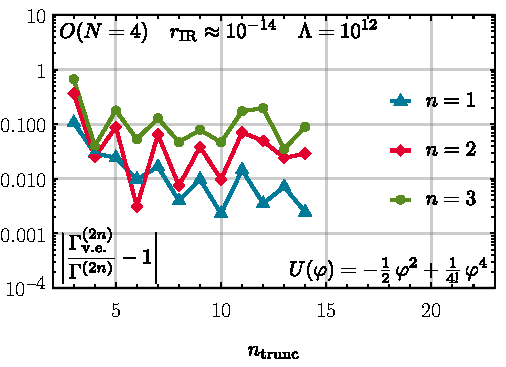
\includegraphics[width=\subcaptionFigureWidth]{0d/figures/sc_ii_n_on_4_lambda_1e12_tir_60_vertex_exp_error.pdf}}% Figure (a)
	{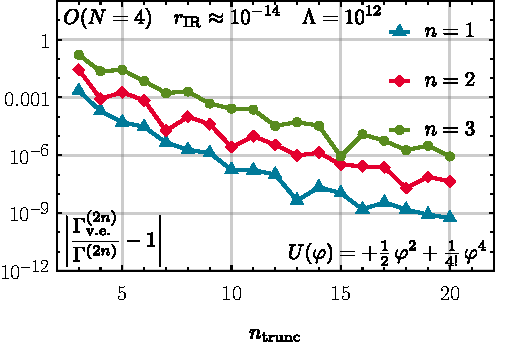
\includegraphics[width=\subcaptionFigureWidth]{0d/figures/sc_ii_p_on_4_lambda_1e12_tir_60_vertex_exp_error.pdf}}% Figure (b)
	[fig:sc_ii_n_on_4_lambda_1e12_tir_60_vertex_exp_error,fig:sc_ii_p_on_4_lambda_1e12_tir_60_vertex_exp_error]% Labels (a) and (b)
	{%
		The relative errors for $\Gamma^{(2n)}$ in the \ir{} for $n = 1, 2, 3$ for the $O (4)$ model, calculated via the \frg{} flow of the Taylor (vertex) expansion to order $m = 2 n_\mathrm{trunc}$ with $n_\mathrm{trunc} \in \{ 3, \ldots , 14 \}$ using the exponential regulator~\eqref{eq:exponential_regulator}.
		As initial condition we use the \uv{} potential \eqref{eq:testing_scenario_phi4} with negative mass term on the left \subref{fig:sc_ii_n_on_4_lambda_1e12_tir_60_vertex_exp_error} and positive mass term on the right \subref{fig:sc_ii_p_on_4_lambda_1e12_tir_60_vertex_exp_error}.
		The discrete results for integer $n_\mathrm{trunc}$ are connected by straight lines to improve readability and for a better trend analysis.
		\fromFigs{24 and 26}{zerod1}%
	}% Caption
	{fig:sc_ii_np_on_4_lambda_1e12_tir_60_vertex_exp_error}% Label	
\paragraph{\frg{} Taylor expansion: $\phi^4$ potential with positive mass term}\phantomsection\label{paragraph:sc2taylorPhiP}\mbox{}\\
We continue our discussion of the \frg{} Taylor expansion by considering the \ic{} \eqref{eq:testing_scenario_phi4} with a positive mass term $+\tfrac{1}{2} \, \vec{\varphi}^{\vts 2}$ and therefore without a non-trivial minimum.
In the context of zero-dimensional $O(N)$ models this \ic{} is in the family of \uv{} potentials discussed qualitatively at length and to some extent even quantitatively in \ccite{Keitel:2011pn,Rosa:2016czs,Moroz:2011thesis}.

In \cref{fig:sc_ii_p_on_4_lambda_1e12_tir_60_vertex_exp_error} we show relative errors for the first three non-vanishing $\Gamma^{(2n)}$ as a function of $n_\mathrm{trunc}$ for this \ic{} for the $O(4)$ model.
These results where obtained using \textit{NDSolve} of \WAMXIIwR{} with an increased \textit{PrecisionGoal} and \textit{AccuracyGoal} of $12$, which became necessary for a proper truncation-error scaling beyond $n_\mathrm{trunc}=15$ for the two-point function.
In \cref{fig:sc_ii_p_on_4_lambda_1e12_tir_60_vertex_exp_error} we observe a truncation-error scaling following power laws in $n_\mathrm{trunc}$ with approximately $n_\mathrm{trunc}^{-8.2}$, $n_\mathrm{trunc}^{-7.6}$, and $n_\mathrm{trunc}^{-7.3}$ for the two-point, four-point, and six-point function respectively.
For this \ic{} the expansion point $\vec{\varphi} = 0$ is located at the global minimum of the potential and the potential is also convex for all $t$.
The dynamics of the \frg{} flow is rather unspectacular for this potential, see Fig.\ 13 of \ccite{Keitel:2011pn} or \cref{fig:sc_ii_p_on=1_n=800_xmax=10_lambda=1.0e12_tir=60_rg_flow} for a visualization.
For the two- and four-point functions, the numerical results at $n_\mathrm{trunc}=3$ ($\Leftrightarrow m=6$) have already acceptable relative errors of $\approx 2.2 \cdot 10^{-3}$ and $\approx 2.8 \cdot 10^{-2}$, respectively, which was observed and discussed in \ccite{Keitel:2011pn}, where results for the Taylor expansions were presented only up to $n_\mathrm{trunc}=3$.
	
The Taylor expansion outperforms the \ktScheme{} in this setting in terms of relative errors.
The performance and practical applicability of the Taylor expansion seem to depend strongly on the \ic{} under consideration.
We will discuss another analytic \ic{} for the Taylor expansion briefly in the next \cref{subsubsec:sc3}.

\paragraph{\frg{} Taylor expansion: Numerical irreversibility}\phantomsection\label{paragraph:sc2taylorIRR}\mbox{}\\
Before we conclude this subsubsection we will briefly comment on the irreversibility of \grg{} flows when employing the \frg{} Taylor expansion.
We discussed in \cref{subsubsec:conservative_form} that the projection onto a finite set of couplings underlying the \frg{} Taylor expansion theoretically allows for an unphysical reversibility of the \grg{} flow.
The \ode{} systems for the running couplings of the \frg{} Taylor expansion in principle allow for an integration both in positive and negative \rgtime{}-direction.
Thus an unphysical resolution of microphysics from macrophysics \dash{} an inversion of the underlying \rg{} transformations connecting them \dash{} is possible when considering a finite set of couplings $\{\bar{\Gamma}^{(2n)}(t)\}$.

We performed practical test with the $\phi^4$ theory discussed in this subsubsection.
For the $\phi^4$ theory with positive mass term discussed in the previous paragraph a complete inversion of the \frg{} flow (from $t=60$ back to $t=0$ using $\Lambda=10^{12}$) is numerically possible for systems with $n_\mathrm{trunc}<7$ for $N=1$.
For larger systems the strong oscillations of the higher-order couplings prevent a numerical integration from the \ir{} back to the \uv{}.
The \ode{} system becomes numerically unstable when approaching $t\approx 24$ from above.
The recovery of the exact \uv{} \ic{} is very good for small $n_\mathrm{trunc}$ but deteriorates when approaching $n_\mathrm{trunc}=7$.
For the $\phi^4$ theory with positive mass term this situations remains qualitatively unchanged for higher $N>1$.

For the $\phi^4$ theory with negative mass term an inversion of the \frg{} flow from the \ir{} to the \uv{} is numerically impossible.
We were not able to find a $n_\mathrm{trunc}$ and $N$ in heuristic tests which allowed for a numerical inversion of the \frg{} flow from $t=60$ back to $t=0$ using $\Lambda=10^{12}$.
The dynamics related to the vaporization of the non-trivial minimum seems to prevent a numerical inversion.
In our heuristic tests it has proven impossible to form back the non-trivial minimum when approaching the \uv{} from the \ir{}.
This is a rather interesting observation which might warrant a detailed investigation of the \ode{} systems involved in the \frg{} Taylor expansion.
Further investigations in higher-dimensional models might be interesting in this context.\bigskip

We will conclude our discussion of the \frg{} Taylor expansion in the next subsubsection with the paragraph \customref{paragraph:sc3taylorConclusion}{FRG Taylor expansion: Concluding remarks}.